

\tikzset{every picture/.style={line width=0.75pt}} %set default line width to 0.75pt        

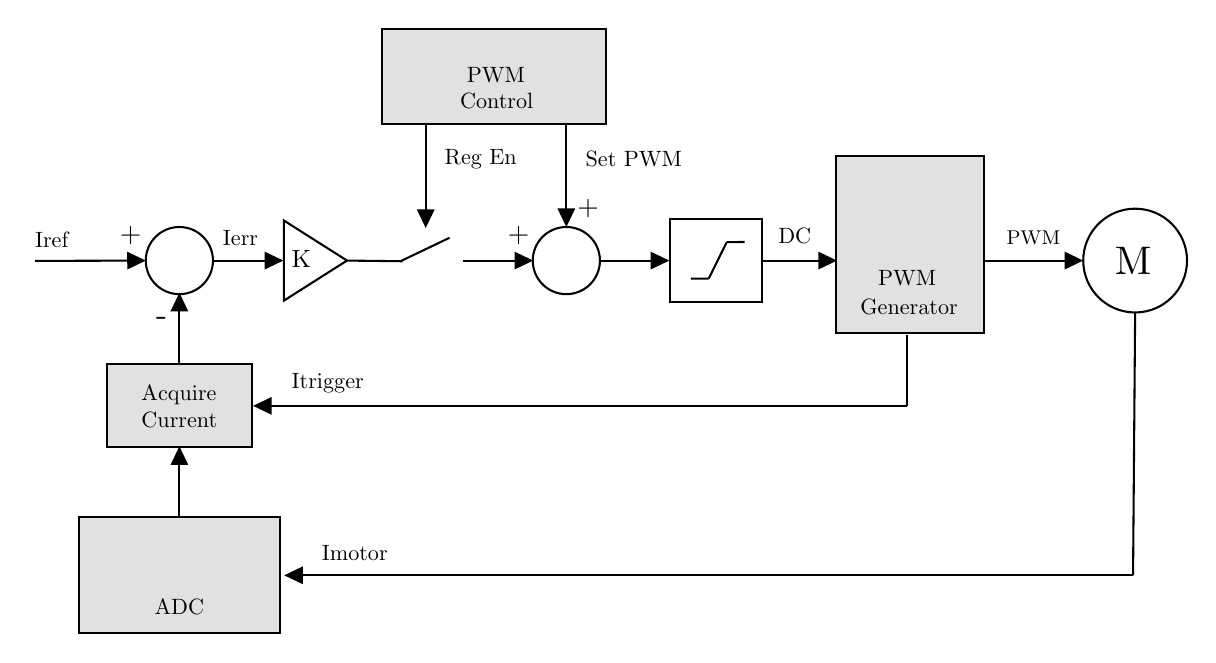
\begin{tikzpicture}[x=0.75pt,y=0.75pt,yscale=-1,xscale=1]
%uncomment if require: \path (0,300); %set diagram left start at 0, and has height of 300

%Shape: Circle [id:dp75942846606901] 
\draw   (130.33,112) .. controls (130.33,103.06) and (137.58,95.82) .. (146.52,95.82) .. controls (155.45,95.82) and (162.7,103.06) .. (162.7,112) .. controls (162.7,120.94) and (155.45,128.18) .. (146.52,128.18) .. controls (137.58,128.18) and (130.33,120.94) .. (130.33,112) -- cycle ;
%Straight Lines [id:da27986909082362965] 
\draw    (146.52,162.21) -- (146.52,130.5) ;
\draw [shift={(146.52,127.5)}, rotate = 450] [fill={rgb, 255:red, 0; green, 0; blue, 0 }  ][line width=0.08]  [draw opacity=0] (8.93,-4.29) -- (0,0) -- (8.93,4.29) -- cycle    ;

%Straight Lines [id:da6600230288463764] 
\draw    (77.05,112.16) -- (127.33,112.01) ;
\draw [shift={(130.33,112)}, rotate = 539.8299999999999] [fill={rgb, 255:red, 0; green, 0; blue, 0 }  ][line width=0.08]  [draw opacity=0] (8.93,-4.29) -- (0,0) -- (8.93,4.29) -- cycle    ;

%Shape: Rectangle [id:dp714942454713728] 
\draw  [fill={rgb, 255:red, 225; green, 225; blue, 225 }  ,fill opacity=1 ] (463,61.52) -- (534.05,61.52) -- (534.05,147) -- (463,147) -- cycle ;
%Shape: Triangle [id:dp4366865800134343] 
\draw   (227.28,112) -- (196.84,131.32) -- (196.84,92.68) -- cycle ;
%Straight Lines [id:da3696616039173719] 
\draw    (227.28,112) -- (254.05,112.32) ;


%Straight Lines [id:da9691180490319533] 
\draw    (253.71,112) -- (276.71,101) ;


%Straight Lines [id:da2520686052851293] 
\draw    (283.36,112) -- (313.98,112) ;
\draw [shift={(316.98,112)}, rotate = 180] [fill={rgb, 255:red, 0; green, 0; blue, 0 }  ][line width=0.08]  [draw opacity=0] (8.93,-4.29) -- (0,0) -- (8.93,4.29) -- cycle    ;

%Shape: Rectangle [id:dp24319017769923046] 
\draw   (382.9,92) -- (427,92) -- (427,132) -- (382.9,132) -- cycle ;
%Straight Lines [id:da7467210515424787] 
\draw    (401.56,120.66) -- (410.24,103.1) ;


%Straight Lines [id:da9410268597126219] 
\draw    (410.24,103.1) -- (418.83,103.05) ;


%Straight Lines [id:da8375418901691511] 
\draw    (392.96,120.71) -- (401.56,120.66) ;



%Straight Lines [id:da7342599903712179] 
\draw    (427.34,112) -- (460.34,112) ;
\draw [shift={(463.34,112)}, rotate = 180] [fill={rgb, 255:red, 0; green, 0; blue, 0 }  ][line width=0.08]  [draw opacity=0] (8.93,-4.29) -- (0,0) -- (8.93,4.29) -- cycle    ;

%Straight Lines [id:da296371673100567] 
\draw    (265.21,46.09) -- (265.21,93.32) ;
\draw [shift={(265.21,96.32)}, rotate = 270] [fill={rgb, 255:red, 0; green, 0; blue, 0 }  ][line width=0.08]  [draw opacity=0] (8.93,-4.29) -- (0,0) -- (8.93,4.29) -- cycle    ;

%Shape: Rectangle [id:dp9289257972427081] 
\draw  [fill={rgb, 255:red, 225; green, 225; blue, 225 }  ,fill opacity=1 ] (244.05,0.29) -- (351.94,0.29) -- (351.94,46) -- (244.05,46) -- cycle ;
%Shape: Circle [id:dp49019498566872044] 
\draw   (316.78,112) .. controls (316.78,103.06) and (324.02,95.82) .. (332.96,95.82) .. controls (341.9,95.82) and (349.14,103.06) .. (349.14,112) .. controls (349.14,120.94) and (341.9,128.18) .. (332.96,128.18) .. controls (324.02,128.18) and (316.78,120.94) .. (316.78,112) -- cycle ;
%Straight Lines [id:da140038158148579] 
\draw    (332.96,46.09) -- (332.96,92.82) ;
\draw [shift={(332.96,95.82)}, rotate = 270] [fill={rgb, 255:red, 0; green, 0; blue, 0 }  ][line width=0.08]  [draw opacity=0] (8.93,-4.29) -- (0,0) -- (8.93,4.29) -- cycle    ;

%Straight Lines [id:da6535254105925976] 
\draw    (162.96,112) -- (193.58,112) ;
\draw [shift={(196.58,112)}, rotate = 180] [fill={rgb, 255:red, 0; green, 0; blue, 0 }  ][line width=0.08]  [draw opacity=0] (8.93,-4.29) -- (0,0) -- (8.93,4.29) -- cycle    ;

%Straight Lines [id:da8262984100189177] 
\draw    (348.94,112) -- (379.55,112) ;
\draw [shift={(382.55,112)}, rotate = 180] [fill={rgb, 255:red, 0; green, 0; blue, 0 }  ][line width=0.08]  [draw opacity=0] (8.93,-4.29) -- (0,0) -- (8.93,4.29) -- cycle    ;

%Shape: Circle [id:dp25249517388379217] 
\draw   (582,112) .. controls (582,98.19) and (593.19,87) .. (607,87) .. controls (620.81,87) and (632,98.19) .. (632,112) .. controls (632,125.81) and (620.81,137) .. (607,137) .. controls (593.19,137) and (582,125.81) .. (582,112) -- cycle ;

%Straight Lines [id:da6638712668031186] 
\draw    (534.34,112) -- (579,112) ;
\draw [shift={(582,112)}, rotate = 180] [fill={rgb, 255:red, 0; green, 0; blue, 0 }  ][line width=0.08]  [draw opacity=0] (8.93,-4.29) -- (0,0) -- (8.93,4.29) -- cycle    ;

%Shape: Rectangle [id:dp6025687451357558] 
\draw  [fill={rgb, 255:red, 225; green, 225; blue, 225 }  ,fill opacity=1 ] (111.52,162) -- (181.52,162) -- (181.52,202) -- (111.52,202) -- cycle ;
%Shape: Rectangle [id:dp6368460798569435] 
\draw  [fill={rgb, 255:red, 225; green, 225; blue, 225 }  ,fill opacity=1 ] (98.03,235.64) -- (195,235.64) -- (195,291.64) -- (98.03,291.64) -- cycle ;
%Straight Lines [id:da3095935870834763] 
\draw    (146.52,236.21) -- (146.52,204.5) ;
\draw [shift={(146.52,201.5)}, rotate = 450] [fill={rgb, 255:red, 0; green, 0; blue, 0 }  ][line width=0.08]  [draw opacity=0] (8.93,-4.29) -- (0,0) -- (8.93,4.29) -- cycle    ;

%Straight Lines [id:da7119757417617545] 
\draw    (497.15,182) -- (185.05,182) ;
\draw [shift={(182.05,182)}, rotate = 360] [fill={rgb, 255:red, 0; green, 0; blue, 0 }  ][line width=0.08]  [draw opacity=0] (8.93,-4.29) -- (0,0) -- (8.93,4.29) -- cycle    ;

%Straight Lines [id:da555961758391875] 
\draw    (606,263.64) -- (200.05,263.64) ;
\draw [shift={(197.05,263.64)}, rotate = 360] [fill={rgb, 255:red, 0; green, 0; blue, 0 }  ][line width=0.08]  [draw opacity=0] (8.93,-4.29) -- (0,0) -- (8.93,4.29) -- cycle    ;

%Straight Lines [id:da5618757081316239] 
\draw    (606,263.64) -- (607,137) ;


%Straight Lines [id:da9238020071399877] 
\draw    (497.15,182) -- (497.15,147.64) ;



% Text Node
\draw (123,100.16) node  [scale=1] [align=left] {+};
% Text Node
\draw (138.02,140) node  [scale=1.2] [align=left] {\mbox{-}};
% Text Node
\draw (85,102) node  [scale=0.8] [align=left] {Iref};
% Text Node
\draw (205.21,111) node  [scale=0.9] [align=left] {K};
% Text Node
\draw (497.15,120.52) node  [scale=0.8] [align=left] {PWM};
% Text Node
\draw (498.1,134.52) node  [scale=0.8] [align=left] {Generator};
% Text Node
\draw (299.42,35.09) node  [scale=0.8] [align=left] {Control};
% Text Node
\draw (298.99,22.49) node  [scale=0.8] [align=left] {PWM};
% Text Node
\draw (558,101.16) node  [scale=0.8] [align=left] {{\small PWM}};
% Text Node
\draw (606,112) node  [scale=1.44] [align=left] {M};
% Text Node
\draw (443,100) node  [scale=0.8] [align=left] {DC};
% Text Node
\draw (146.52,182.33) node  [scale=0.8] [align=left] {Acquire\\Current};
% Text Node
\draw (146.52,279) node  [scale=0.8] [align=left] {ADC};
% Text Node
\draw (310,100.16) node  [scale=1] [align=left] {+};
% Text Node
\draw (343.46,87.16) node  [scale=1] [align=left] {+};
% Text Node
\draw (365.46,63) node  [scale=0.8] [align=left] {Set PWM};
% Text Node
\draw (291.71,63) node  [scale=0.8] [align=left] {Reg En};
% Text Node
\draw (176,101.16) node  [scale=0.8] [align=left] {Ierr};
% Text Node
\draw (218,171) node  [scale=0.8] [align=left] {Itrigger};
% Text Node
\draw (231.02,252.64) node  [scale=0.8] [align=left] {Imotor};


\end{tikzpicture}
